\documentclass[12pt]{article}
%% Insert Commands in Preface.tex
\addtolength{\hoffset}{-2.25cm}
\addtolength{\textwidth}{4.5cm}
\addtolength{\voffset}{-2.5cm}
\addtolength{\textheight}{5cm}
\setlength{\parskip}{0pt}
\setlength{\parindent}{15pt}

\usepackage{amsthm, amsmath, amssymb, mathbbol}
\usepackage[colorlinks = true, linkcolor = black, citecolor = black, final]{hyperref}

\newtheorem{theorem}{Theorem}[section]
\newtheorem{corollary}[theorem]{Corollary}
\newtheorem{lemma}[theorem]{Lemma}
\newtheorem{example}[theorem]{Example}
\newtheorem{definition}[theorem]{Definition}

\usepackage{mathrsfs}
\usepackage{graphicx}
\usepackage{multicol}
\usepackage{accents}
\usepackage{tikz}
\usepackage{xcolor}
\usetikzlibrary{patterns}

\setlength{\parindent}{0in}

\pagestyle{empty}

%% Insert Commands Below This Line


\begin{document}

\thispagestyle{empty}

{\scshape Huang Linhang; Syx Pek; Qi Ji} \hfill {\scshape \large Differential Geometry} \hfill {\scshape Homework \#1}

\smallskip
\hrule
\bigskip

\section{Section 1.3}

\subsection*{Question 2}

A circular disk of radius 1 in the plane $xy$ rolls without slipping along the x
axis. The figure described by a point of the circumference of the disk is calIed a
cycloid.

\begin{itemize}
     \item Obtain a parametrized curve $\alpha : \mathbb{R} \to \mathbb{R}^2$ the trace of which is the cycloid,
and determine its singular points.
     \item Compute the arc length of the cycloid corresponding to a complete rotation
     of the disk.
\end{itemize}

Solution:

Let us first parameterize the location of the centre of the 
circle. When it has rotated by $\theta$, it will also have moved $\theta$ to the right.
Hence, the position of the centre with respect to amount of rotation is $(\theta, 1)$.

Now consider the positional vector from the centre to the marked point
on the circumference. At $\theta = 0$, this is at $(0, -1)$. Then, for general $\theta$, 
this is at $(-\sin\theta, -\cos\theta)$. Summing this, it shows that the parameterization $\alpha(\theta) = (\theta - \sin\theta, 1 - \cos\theta)$.

We shall use the arc-length formula to yield

\begin{align*}
     \int_0^{2\pi} |\nabla\alpha(x)| \mathrm{d}x 
     &= \int_0^{2\pi} \sqrt{(1-\cos x)^2 + (\sin x)^2} \mathrm{d}x  \\
     &=\int_0^{2\pi} \sqrt{2 - 2\cos{x}} \mathrm{d}x \\
     &= \left[-4\cos{\frac x2}\right]^{x = 2\pi}_{x = 0} \\
     &= 8.
\end{align*}

\subsection*{Question 3}

From errata: p.~8, Figure 1-8: The labelling is wrong: the points \(p\)
and \(C\) should lie on the same half-line \(r\) through \(0\) as \(B\).

Let \(0A = 2a\) be the diameter of a circle \(S^1\) and \(0Y\) and
\(AV\) be the tangents to \(S^1\) at \(0\) and \(A\), respectively. A
half-line \(r\) is drawn from \(0\) which meets the circle \(S^1\) at
\(C\) and the line \(AV\) at \(B\). On \(0B\) mark off the segment
\(0p = CB\) (means both segments are equally long). If we rotate \(r\)
about \(0\), the point \(p\) will describe a curve called \emph{cissoid
of Diocles}. By taking \(0A\) as \(x\) axis and \(0Y\) as \(y\) axis,
prove that

\begin{enumerate}
\def\labelenumi{\alph{enumi}.}
\item
  The trace of
  \[ \alpha(t) = \left( \frac{2at^2}{1+t^2}, \frac{2at^3}{1+t^2} \right) ,\quad t\in\mathbb{R} \]
  is the cissoid of Diocles (\(t = \tan\theta\), see Figure 1-8)
\end{enumerate}

\emph{Proof.}

\begin{figure} \label{Pic}
     \center
     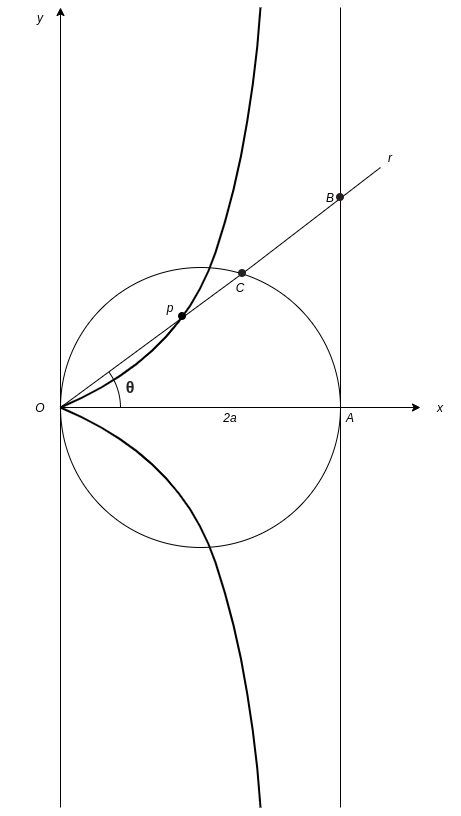
\includegraphics[scale = 0.3]{Untitled Diagram.png}
\end{figure}

Let \(t = \tan\theta\) for \(\theta \in (-\pi,\pi)\), fix \(\theta\) and
we show that \(p = \alpha(\tan\theta)\) satisfies the requirements when
the half line \(r\) is of angle \(\theta\) from origin. Refer to Figure \ref{Pic}

First we check that \(p\) lies on the half-line, where
\[ p = \left( \frac{2a\tan^2\theta}{1+\tan^2\theta}, \frac{2a\tan^3\theta}{1+\tan^2\theta} \right) \]
and we see that \(\tan\arg p = \tan\theta\).

Finally we check that the segments \(0p = CB\), we know the point \(C\)
can be given by \((a,0) + (a \cos 2\theta, a \sin 2\theta)\) and \(B\)
is given by \((2a, 2a\tan\theta )\). So \begin{align*}
\left\lVert CB \right\rVert &= \left\lVert \left(  a - a\cos 2\theta, 2a\tan\theta - a\sin 2\theta  \right) \right\rVert \\
\left\lVert CB \right\rVert^2 &=
(a - a\cos2\theta)^2 + (2a\tan\theta - a\sin2\theta)^2 \\
&= 4a^2\sin^2\theta\tan^2\theta \\
\left\lVert p \right\rVert^2 &= \frac{4a^2(t^4 + t^6)}{(1+t^2)^2} \\
&= \frac{4a^2 \tan^4\theta}{1+\tan^2\theta} \\
&= 4a^2\sin^2\theta\tan^2\theta
\end{align*}

\begin{enumerate}
\def\labelenumi{\alph{enumi}.}
\setcounter{enumi}{1}
\item
  The origin \((0,0)\) is a singular point of the cissoid.
\end{enumerate}

\emph{Proof.} At point \((0,0)\), \(t = 0\), we just need to check that
\(\alpha'(0) = 0\). Now
\[ \alpha'(t) = \left( \frac{4a t}{(1+t^2)^2}, \frac{2a t^2(t^2 + 3)}{(1+t^2)^2}  \right) \]
which is \(0\) when \(t = 0\).

\begin{enumerate}
\def\labelenumi{\alph{enumi}.}
\setcounter{enumi}{2}
\item
  As \(t\to\infty\), \(\alpha(t)\) approaches the line \(x = 2a\), and
  \(\alpha'(t) \to (0, 2a)\) (book typo'd this I think). Thus as
  \(t\to\infty\), the curve and its tangent approach the line
  \(x = 2a\).
\end{enumerate}

\emph{Proof.} To show that the curve approaches the line \(x=2a\) we
check that \[ \lim_{t\to\infty} \frac{2at^2}{1+t^2} = 2a. \] To verify
the other claim we compute \[ \lim_{t\to\infty} \alpha'(t) = (0, 2a). \]


\subsection*{Question 4}

Let $\alpha : (0, \pi) \to \mathbb R^2$ be given by
$$\alpha(t) = \left ({\color{red}\sin t}, \cos t + \log \tan \frac t2\right )$$
where $t$ is the angle that the $y$ axis makes with the vector $\alpha(t)$. The trace of $\alpha$ is
called the tractrix. 
Show that

(a) $\alpha$ is a differentiable parameterized curve, regular except $t = \frac \pi2$.
Consider the derivative, $\alpha'(t) = \left (\cos t, -\sin t + (\sin t)^{-1}\right )$
This is differentiable except when $\cos t = 0$ and $-\sin t + (\sin t)^{-1} = 0$, 
which occurs when $t = \frac \pi2$.

(b) The length of the segment of the tangent of the tractrix 
between the point of tangency and the $y$ axis is constantly equal to 1.

Consider $\frac {\alpha'(t)_y}{\alpha'(t)_x} = \frac{-\sin t + (\sin t)^{-1}}{\cos t} = \frac {\cos t}{\sin t}.$ This is as $(\sin x)^2 + (\cos x)^2 = 1.$
Thus, the line of the tanget at $\alpha(t)$ is $y - \cos t - \log \tan \frac t2 = \frac{\cos t}{\sin t}(x - \sin t).$
This has $y$-intersect $(0,\log \tan \frac t2).$ Then, the distance is $(\sin t)^2 + (\cos t + \log \tan \frac t2 - \log \tan \frac t2)^2 = 1.$



\subsection*{Question 5}

Let $\alpha : (-1, \infty) \to \mathbb{R}^2$ be given by
\begin{equation*}
     \alpha(t) = \left(\frac{3at}{1+t^3},\frac{3at^2}{1+t^3}\right)
\end{equation*}

Solution:

(a) For $t = 0$, $\alpha$ is tangent to the $x$-axis.
Computing the derivative, $\frac{\partial \alpha(t)}{\partial t} = \left(\frac{a(3 - 6t^3)}{(1+t^3)^2},\frac{3at(2-t^3)}{(1+t^3)^2}\right)$.
Thus, $\alpha(0) = (0,0)$ and $\frac{\partial \alpha(0)}{\partial t} = (3a, 0)$. Thus, it is tangent to the $x$-axis.

(b) As $t \to \infty$, $\alpha(t) = \frac{\partial \alpha(t)}{\partial t} = (0,0).$
We take limits, $\lim_{t\to \infty}\alpha(t) = \left(\lim_{t\to \infty}\frac{3at}{1+t^3},\lim_{t\to\infty}\frac{3at^2}{1+t^3}\right) = (0,0).$
Similarly, $\lim_{t \to \infty} \frac{\partial \alpha(t)}{\partial t} = 
\left(\lim_{t\to \infty}\frac{a(3 - 6t^3)}{(1+t^3)^2},\lim_{t\to \infty}\frac{3at(2-t^3)}{(1+t^3)^2}\right) = (0,0).$

(c)Take the curve with the opposite orientation. 
Now, as $t \to -1$, the curve
and its tangent approach the line $x + y + a = 0$.

Let us compute $\lim_{t\to -1}\frac {\alpha(t)_y}{\alpha(t)_x} = \lim_{t\to -1} \frac 1t = -1.$
Now, consider $$\lim_{t \to -1} \alpha(t)_y - (-1)\alpha(t)_x = \lim_{t\to -1} \frac{3a(t + t^2)}{1 + t^3} = -a.$$

Also $\lim_{t\to -1}\frac {\alpha'(t)_y}{\alpha'(t)_x} = \lim_{t\to -1} \frac{3t(2-t^3)}{3-6t^3} = \frac{-9}{9}=-1$, which is a slope of x+y+a=0.

Thus, the curve and its tangent approach the line $y = (-1)x + (-a)$, or the line $x + y + a = 0.$

\subsection*{Question 10}

Let $\alpha: I \to \mathbb{R}^3$ be a parametrized curve.
Let $[a,b] \subseteq I$ and set $\alpha(a) = p, \alpha(b) = q.$

(a) Show that, for any constant vector $v$, $|v| = 1$.
     \begin{equation*}
          (q-p)\cdot v = \int_a^b \alpha'(t)\cdot v \mathrm{d}t \leq \int_a^b |\alpha'(t)| \mathrm dt.
     \end{equation*}

\begin{proof}
     By Fundamental Theorem of Calculus in 1-Dimension,
     $$\int_a^b \alpha'(t)\cdot v\mathrm dt = (\alpha(b) - \alpha(a))\cdot v = (q-p)\cdot v.$$
     Then, by H\"{o}lder's inequality, we have $|\alpha'(t)\cdot v| \leq |\alpha'(t)||v| = |\alpha'(t)|.$
     Thus, $$\left |\int_a^b \alpha'(t)\cdot v\mathrm dt\right | \leq \int_a^b |\alpha'(t)\cdot v| \mathrm dt \leq \int_a^b |\alpha'(t)| \mathrm dt.$$
\end{proof}

(b) Set $$v = \frac{q-p}{|q-p|}$$ and show that
$$|\alpha(b)-\alpha(a)| \leq \int_a^b |\alpha'(t)|\mathrm dt.$$
That is, the curve of shortest length from $\alpha(a)$ to $\alpha(b)$
is the straight line joining these points.

\begin{corollary}
     Use $(q-p)\cdot v = \frac{|q-p|^2}{|q-p|} = |q-p| = |\alpha(b) - \alpha(a)|$ with 10(a).
\end{corollary}
\section{Section 1.4}

\subsection*{Question 10}
The natural orientation of $R^2$ makes it possible to associate a sign to the area $A$ of a parallelogram generated by two linearly independent vectors $u,v \in R^2$. To do this, let $\{e_i\}, i = 1, 2$, be the natural ordered basis of $R^2$, and write $u = u_1e_1 +u_2e_2, v = v_1e_1 +v_2e_2$. Observe the matrix relation \begin{equation*}
    \begin{pmatrix}
    u \cdot u & u \cdot v\\
    v \cdot u & v \cdot v
    \end{pmatrix} =
    \begin{pmatrix}
    u_1 & u_2\\
    v_1 & v_2
    \end{pmatrix}
    \begin{pmatrix}
    u_1 & v_1\\
    u_2 & v_2
    \end{pmatrix}
\end{equation*}
and conclude that \begin{equation*}
    A^2 = \begin{array}{|cc|}
         u_1 & u_2\\
         v_1 & v_2
    \end{array}^2.
\end{equation*}
Since the last determinant has the same sign as the basis $\{u,v\}$, we can say that $A$ is positive or negative according to whether the orientation of $\{u,v\}$ is positive or negative. This is called the \textit{oriented area} in $R^2$.\\\\
Solution:


We first observe that
  \begin{equation*}
     \begin{pmatrix}
     u \cdot u & u \cdot v\\
     v \cdot u & v \cdot v
     \end{pmatrix} =
     \begin{pmatrix}
          u_1^2 + u_2^2 & u_1v_1 + u_2v_2\\
          v_1u_1 + v_2u_2 & v_1^2 + v^2_2
     \end{pmatrix} = 
     \begin{pmatrix}
     u_1 & u_2\\
     v_1 & v_2
     \end{pmatrix}
     \begin{pmatrix}
     u_1 & v_1\\
     u_2 & v_2
     \end{pmatrix}
 \end{equation*}

 The identity then holds as, 
\begin{align*}
    A^2 &= (u \wedge v) \cdot (u \wedge v)\\
    &= u \cdot (v \wedge (u \wedge v))\\
    &= u \cdot [(v \cdot v)u - (v \cdot u)v]\\
    &= (u \cdot u)(v \cdot v) - (v \cdot u)(v \cdot u)\\
    &= \begin{array}{|cc|}
    u \cdot u & u \cdot v\\
    v \cdot u & v \cdot v
    \end{array}\\
    &= \begin{array}{|cc|}
    u_1 & u_2\\
    v_1 & v_2
    \end{array}~
    \begin{array}{|cc|}
    u_1 & v_1\\
    u_2 & v_2
    \end{array}\\
    &=\begin{array}{|cc|}
    u_1 & u_2\\
    v_1 & v_2
    \end{array}^2.
\end{align*}
\subsection*{Question 11}
a. Show that the volume $V$ of a parallelepiped generated by three linearly independent vectors $u,v,w \in R^3$ is given by $V=|(u \wedge v)\cdot w|$, and introduce an oriented volume in $R^3$.\\
b. Prove that \begin{equation*}
     V^2 = \begin{array}{|ccc|}
     u \cdot u & u \cdot v & u \cdot w\\
     v \cdot u & v \cdot v & v \cdot w\\
     w \cdot u & w \cdot v & w \cdot w
     \end{array}
 \end{equation*}\\\\
Solution.
(a) Let $n = \frac{u \wedge v}{||u \wedge v||}$ be the normal vector of the plane generated by $u$ and $v$. Then \begin{align*}
     V &= (||u||\times||v||\times|\sin(u,v)|)\times||w||\times|\cos(n,w)|\\
     &= ||u\wedge v||\times||w||\times|\cos(n,w)|\\
     &= ||u\wedge v||\times||w||\times|\cos(u\times v,w)|\\
     &= |(u\wedge v)\cdot w|
 \end{align*}
(b) We know that \begin{align*}
     |(u\wedge v)\cdot w| &= |\begin{pmatrix}
     u_2v_3-v_2u_3\\
     u_3v_1-v_3u_1\\
     u_1v_2-v_1u_2
     \end{pmatrix}\cdot w|\\
     &=\begin{array}{|ccc|}
     u_1 & u_2 & u_3\\
     v_1 & v_2 & v_3\\
     w_1 & w_2 & w_3
     \end{array}\\
     &=\det (u,v,w).
 \end{align*}
Hence, \begin{align*}
     V^2 &= \det (u,v,w)^2\\
     &=|\begin{pmatrix}
     u^T\\
     v^T\\
     w^T
     \end{pmatrix}
     \begin{pmatrix}
      u&v&w
     \end{pmatrix}|\\
     &=\begin{array}{|ccc|}
     u^T u & u^T v & u^T w\\
     v^T u & v^T v & v^T w\\
     w^T u & w^T v & w^T w
     \end{array}\\
     &=\begin{array}{|ccc|}
     u \cdot u & u \cdot v & u \cdot w\\
     v \cdot u & v \cdot v & v \cdot w\\
     w \cdot u & w \cdot v & w \cdot w.
     \end{array}
 \end{align*}
\subsection*{Question 12}
Given the vectors $v \neq 0$ and $w$, show that there exists a vector $u$ such that $u \wedge v = w$ if and only if $v$ is perpendicular to $w$. Is this vector $u$ uniquely determined? If not, what is the most general solution?\\\\
Solution: $(\Rightarrow)$ By the properties of cross product, $u \wedge v = w$ implies that $v \cdot w = 0$.

$(\Leftarrow)$ If $v\cdot w=0$, we have \begin{align*}
     (v\wedge w)\wedge v &= (v\cdot v)w - (v\cdot w)v=||v||^2w.
\end{align*}
Then $v\neq 0$ implies that $w = \frac{v\wedge w}{||v||^2}\wedge v$. Let $u=\frac{v\wedge w}{||v||^2}$ and we have $u\wedge v = w$.

Suppose there exist $u'$ other than $u$ such that $u'\times v = w$. Then \begin{align*}
     &u \wedge v = u' \wedge v \\
     \Rightarrow &(u'-u)\wedge v = 0\\
     \Rightarrow &u'-u = kv, \quad k\in R\\
     \Rightarrow &u' = u + kv, \quad k\in R.
\end{align*}

Therefore, the most general solution of $u\wedge v=w$ is 
\begin{equation*}
     u = \frac{v\wedge w}{||v||^2} + kv,\quad k\in R.
\end{equation*}

\end{document}
